\documentclass{article}
\usepackage{geometry}
\usepackage{enumitem}
\usepackage{parskip}
\geometry{
	a4paper,
	total={210mm,297mm},
	left=25mm,
	right=25mm,
	top=25mm,
	bottom=25mm
}
\setlist[description]{leftmargin=\parindent,labelindent=\parindent}
\usepackage[utf8]{inputenc}
\usepackage{graphicx}
\graphicspath{{Bilder/}}

\renewcommand{\contentsname}{Inhaltsverzeichnis}
\begin{document}

\pagenumbering{roman}

\title{Software Projekt - Excel als SQL Datenbank}
\author{Authoren: Rijad \v{Z}u\v{z}o, Séverin Müller \\ \\ Dozent: Ulrich Hauser}

\maketitle

\vspace{80mm}
\begin{center}
		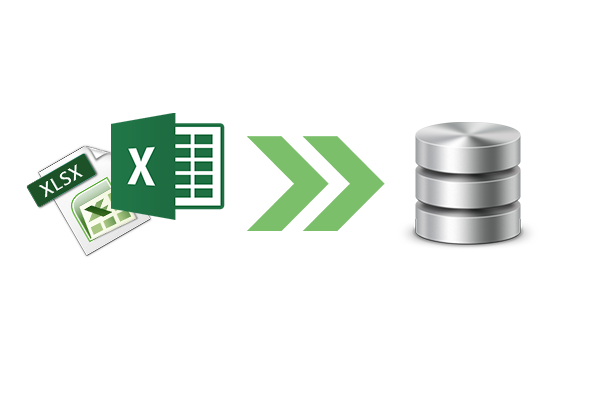
\includegraphics{SoftwareLogo}
\end{center}

\newpage
\tableofcontents
\newpage

\pagenumbering{arabic}

\section{Motivation}
Das Projekt wurde von uns in der Freizeit für den Bosnischen Club St. Gallen erarbeitet. Diese führen seit langem eine Excel-Liste für die Mitgliederverwaltung. \newline 
Für Sie war dies das einfachste Werkzeug, jedoch gab es immer wieder Probleme, wie zum Beispiel das ungewollte löschen ganzer Zeilen, oder das verrutschen in den Zeilen / Spalten. Wir wollten jedoch nicht eine komplett neue Datenbank erarbeiten, und entschieden uns, Ihnen ein Werkzeug für die Verwaltung der vorhandenen Excel Tabelle zur Verfügung zu stellen, welches eine einfache, intuitive GUI zur Verfügung stellt.

\subsection{Ausgangssituation}
Nebst den Problemen bei unaufmerksamer Bearbeitung, ist das Auslesen eines grösseren Excel Files deutlich langsamer als bei einer SQL Datenbank der gleichen bzw. einer vielfachen Grösse, deshalb ist es sinnvoll das Excel File in eine SQL Tabelle umzuwandeln und so zu Verarbeiten. \newline 

Die Konversion würde zusätzliche Software Kenntnisse erfordern, so griffen wir auf Vorhandene Office Werkzeuge zurück. \\

Mit unserer x2dB Applikation wurde das Problem gelöst. Die Umwandlung ist dank ODBC Connector unnötig und somit kann das Excel File bestehend bleiben.

\subsection{Lösungsidee}
Wir legten vor allem Wert auf ein simples User-Interface mit allen nötigen Funktionen. Die Software verarbeitet das Excel File im Hintergrund als SQL Tabelle und verbindet sich mit entsprechenden Treibern über ein File das via GUI eingebunden werden kann. Das ermöglichen uns die Microsoft.Office.Core und Microsoft.Office.Excel.Interop Treiber. \\

Mit unserer Applikation hat der User einen begrenzten Einfluss auf das File und kann so weniger Schaden am File anrichten. Schaden können auch gleichzeitige Lese- / Speicherzugriffe auf ein Shared File auf einem Netzwerklaufwerk. In unserer Applikation dauert die Verbindung nur kurz, bis die Daten gelesen/geschrieben wurden und danach wird das File wieder freigegeben.

Für zusätzliche Datenintegrität wird jeweils ein Backup des Files erstellt und kann nötigen Falls zurück gespielt werden. Dies ist nicht die 'ultimative Lösung', aber wir konnten so die Sicherheit bei Veränderungen am Excel File erhöhen und trotzdem ein 'für jeden lesbares' Dateiformat weiter verwenden, dass zum Beispiel auch mit einem USB Stick übertragen und auf heimischen Computern (weiter-)bearbeitet werden kann.

\section{Anforderungsliste}
Um die Bedürfnisse der Verwalter dieser Excel Liste bestmöglich abdecken zu können, haben wir uns mit Ihnen zusammen gesetzt und die nachfolgenden Anforderungen definiert. 
	
\subsection{Muss-Anforderungen}
Die Applikation muss:
	\begin{description}
		\item[M1:] Das vorhandene Excel File als Datenbasis verwenden.
		\item[M2:] Das Excel File lesen und beschreiben können.
		\item[M3:] Nach dem Lesen bzw. Schreiben die Verbindung trennen.
		\item[M4:] In regelmässigen Abständen Backups erstellen.
	\end{description}

\subsection{Soll-Anforderung}
Die Applikation soll:
\begin{description}
	\item[S1:] Leicht Bedienbar sein.
	\item[S2:] Ein intuitives, einfaches User-Interface haben.
	\item[S3:] Dem User das Handling des Excel Files abnehmen.
\end{description}

\subsection{Wunsch-Anforderung}
Die Applikation könnte:
\begin{description}
	\item[W1:] Eine Benutzungsanleitung haben.
	\item[W2:] Mehrere Sprachen unterstützen.
	\item[W3:] Dem User Hilfe anbieten.
\end{description}

\newpage

\section{Projektumgebung}
\vspace{5mm}
\subsection{Entwicklungsprozess	}
Da es sich um eine Applikation handelt welche eng mit dem User verbunden ist kann es auch //TODO SCRUM

\subsection{Programmiersprache}
Die Excel Software lauft ausschließlich auf Microsoft Windows Betriebssystemen, deshalb haben wir uns für die Windows Spezifische Programmiersprache C\# entschieden. \\ Diese in Kombination mit der IDE Visual Studio ermöglichten uns eine angenehme Entwicklung sowohl der Funktionalität und auch des GUI's.

asdkljfasökldfjasöklfjasdöklfjökl
 

\subsection{Verwaltungssystem}
Die Auswahl des Verwaltungssystem war sehr einfach da wir die Software als Open Source ausgeben wollten. Wir haben uns für das Git System entschieden und hosteten unser code auf der Website GitHub.

\newpage

\section{Projekt Planung}
\subsection{Product Backlog}
\subsection{Sprints}
\subsection{Sprint Stand-up Meetings}
\subsection{Sprint Review}

\newpage

\section{Ablauf der Entwicklung}

\subsection{Modellierung}
Die erste Phase der Entwicklung war das Strukturieren der Software. Wir wollten ein klares Design haben das uns die Weiterentwicklung in der Zukunft ermöglicht. 

\subsubsection{Klassen Diagramm}
\begin{center}
	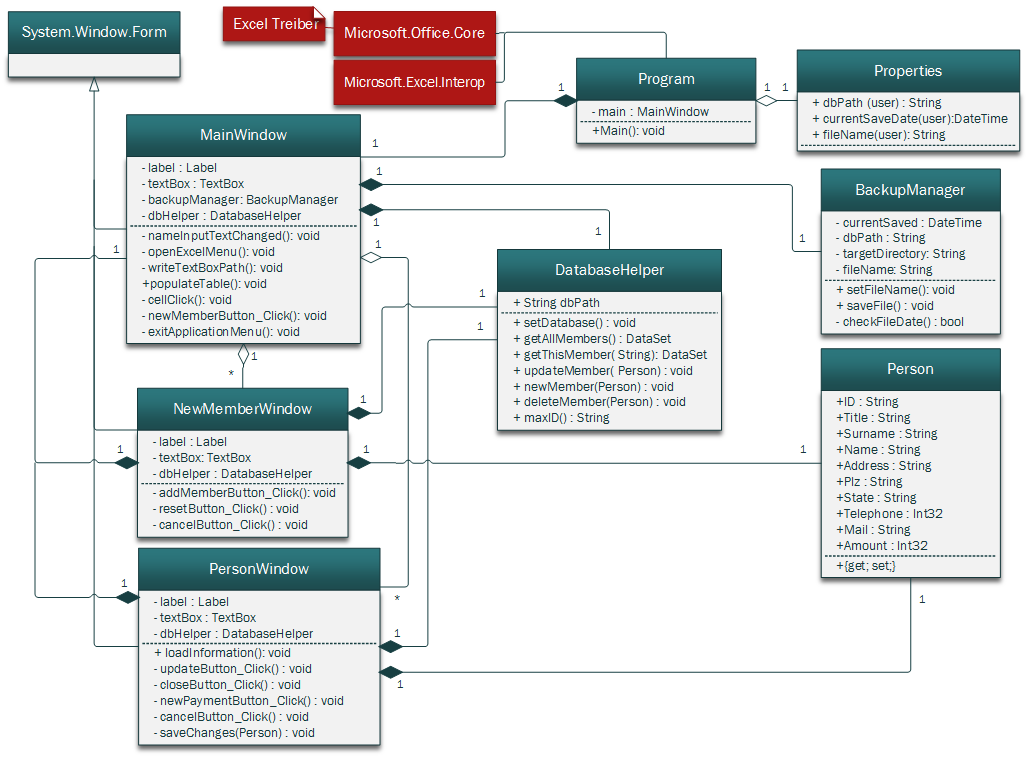
\includegraphics[width=1.05 \textwidth]{KlassendiagrammBild}
	\caption{1.a Klassendiagramm}
\end{center}

\subsubsection{Aktivitäts-Diagramm}

\subsubsection{Sequenz Diagramm}

\subsection{Stunden Journal}
Bild oder tabelle rekreiren von der Stunden template vom Sevi.

\subsection{GUI}
Vorgang bei Gestaltung des GUI's, bedenken usw.

\subsection{Database Handling}
Schwierigkeiten bei den Referenzen, Voraussetzungen zur Verbindung usw.

\subsection{Backup Management}
Ansätze für ein effizientes Backuping :).

\subsection{Testen}
Wie beim Testen vorgegangen wurde!

\newpage

\section{Ziel}
\subsection{Resultat}


\end{document}